\documentclass[11pt,usenames,dvipsnames,svgnames,x11names]{beamer} 

\usetheme{Singapore}
\usepackage{amssymb,amsmath,amsthm,amsfonts}                    
\usecolortheme{dolphin} 
\setbeamertemplate{navigation symbols}{}
\usepackage[utf8]{inputenc} 
\usepackage{polski}
\usepackage{tikz}
\usepackage{subfigure}
\usepackage{setspace}
\usepackage{savesym}
\savesymbol{arc}
\usepackage{color}
\usepackage{xcolor}
\usepackage{pict2e}
\usepackage{epstopdf}
\usepackage{caption}
\usepackage{graphicx}
\usepackage{pict2e}
\usepackage{epstopdf}
\usepackage{geometry}
\usepackage{mathabx}
\usepackage[normalem]{ulem}
\usepackage{wrapfig}
\usepackage{multirow}
\usepackage{booktabs}
\usepackage{pifont}
% \usepackage{picins}
% \usepackage{floatflt}

\title{STATYSTYCZNE METODY \newline REGRESJI PORZĄDKOWEJ}
\author{Marta Sommer}
\institute{MiNI, Politechnika Warszawska}
\titlegraphic{
\includegraphics[scale=0.5]{mini.jpg}}
\date{10 marca 2015}

\renewcommand*{\tablename}{Wykres}
\theoremstyle{plain}
\newtheorem{twierdzenie}{Twierdzenie} 
\newtheorem{twierdzeniecd}{Twierdzenie cd.} 
\theoremstyle{definition}
\newtheorem{definicja}{Definicja}
\newtheorem{przyklad}{Przykład}
\newtheorem{lemat}{Lemat}
\newtheorem{wniosek}{Wniosek}
\newtheorem{oznaczenia}{Oznaczenia}
\theoremstyle{remark}
\newtheorem{uwaga}{Uwaga}
\renewcommand*{\figurename}{Figure} 

\setbeamertemplate{caption}[numbered]
\setbeamertemplate{footline}[frame number]

\begin{document}

\begin{frame}
	\titlepage
\end{frame}

%%%%%%%%%%%%%%%%%%%%%%%%%%%%%%%%%%%%%%%%%%%%%%%%%%%%%%%%%%%%%%%%%%%%%%%%%%%%%%%%%%%%%%%%%%%%%%%%%%%%%%%%%%%%%%%%%%%%%

\begin{frame}
\Huge
\centering
\textbf{PRZYKŁAD}
\end{frame}

\begin{frame}
Załóżmy, że chcemy modelować zmienną odpowiedzi przyjmującą wartości ze zbioru: 
\begin{eqnarray*}
\mathcal{Y}=&\lbrace&\hspace{0mm}bardzo\_sie\_nie\_zgadzam,\hspace{5mm}nie\_zgadzam\_sie,\\ && zgadzam\_sie,\hspace{5mm}bardzo\_sie\_zgadzam\hspace{3mm} \rbrace.
\end{eqnarray*}

W naturalny sposób są to dane uporządkowane:
\begin{eqnarray*}
bardzo\_sie\_nie\_zgadzam &\prec& nie\_zgadzam\_sie\hspace{3mm}\prec \\
\prec\hspace{3mm}zgadzam\_sie &\prec& bardzo\_sie\_zgadzam.
\end{eqnarray*} 
Mamy też dane zmienne objaśniające - oznaczmy je standardowo przez $\mathcal{X}$.  
\end{frame}

\begin{frame}
\Huge
\centering
\textbf{MODEL PROPORCJONALNYCH SZANS}
\end{frame}

\begin{frame}
Interesują nas:
$$
\Pi_j(\underline{x})=\mathbb{P}(Y=j\hspace{1mm}|\hspace{1mm}\underline{x}),\hspace{2cm} \textrm{dla}\hspace{3mm} j=1,\ldots,J.
$$
Rozważamy skumulowane prawdopodobieństwa:
$$
\mathbb{P}(Y\leq j \hspace{1mm}|\hspace{1mm} \underline{x})=\Pi_1(\underline{x})+\ldots+\Pi_j(\underline{x}).
$$
Oraz model:
$$
\log\dfrac{\mathbb{P}(Y\leq j \hspace{1mm}|\hspace{1mm} \underline{x})}{\mathbb{P}(Y> j \hspace{1mm}|\hspace{1mm} \underline{x})} = \alpha_j+\underline{\beta}'\underline{x}.
$$
Współczynniki wyliczamy metodą Raphsona-Newtona, a szukane prawdopodobieństwa - po prostym przeliczeniu - dostaniemy ze~wzoru:
$$
\mathbb{P}(Y\leq j \hspace{1mm}|\hspace{1mm} \underline{x})=\dfrac{e^{\alpha_j+\underline{\beta}'\underline{x}}}{1+e^{\alpha_j+\underline{\beta}'\underline{x}}}.
$$ 
\end{frame}

\begin{frame}
\Huge
\centering
\textbf{WEKTORY MASZYN PODPIERAJĄCYCH (SVM)}
\end{frame}

\begin{frame}
\frametitle{\small PRZYPADEK DWUKLASOWY, LINIOWO SEPAROWALNY}
%Konstruujemy dwie równoległe i maksymalnie oddalone od siebie hiperpłaszczyzny, we wnętrzu których nie leży ani jeden element próby uczącej. Ich równania %to:
\begin{columns}
\begin{column}[t]{0.5\textwidth}
Konstruujemy dwie równoległe i~maksymalnie oddalone od~siebie hiperpłaszczyzny, we~wnętrzu których nie~leży ani~jeden element próby uczącej. Ich równania~to:
$$
\begin{cases}
x'_i\textbf{w}+b &= 1\\
x'_i\textbf{w}+b &= -1
\end{cases}
$$
\end{column}
\begin{column}[t]{0.5\textwidth}
\begin{center}
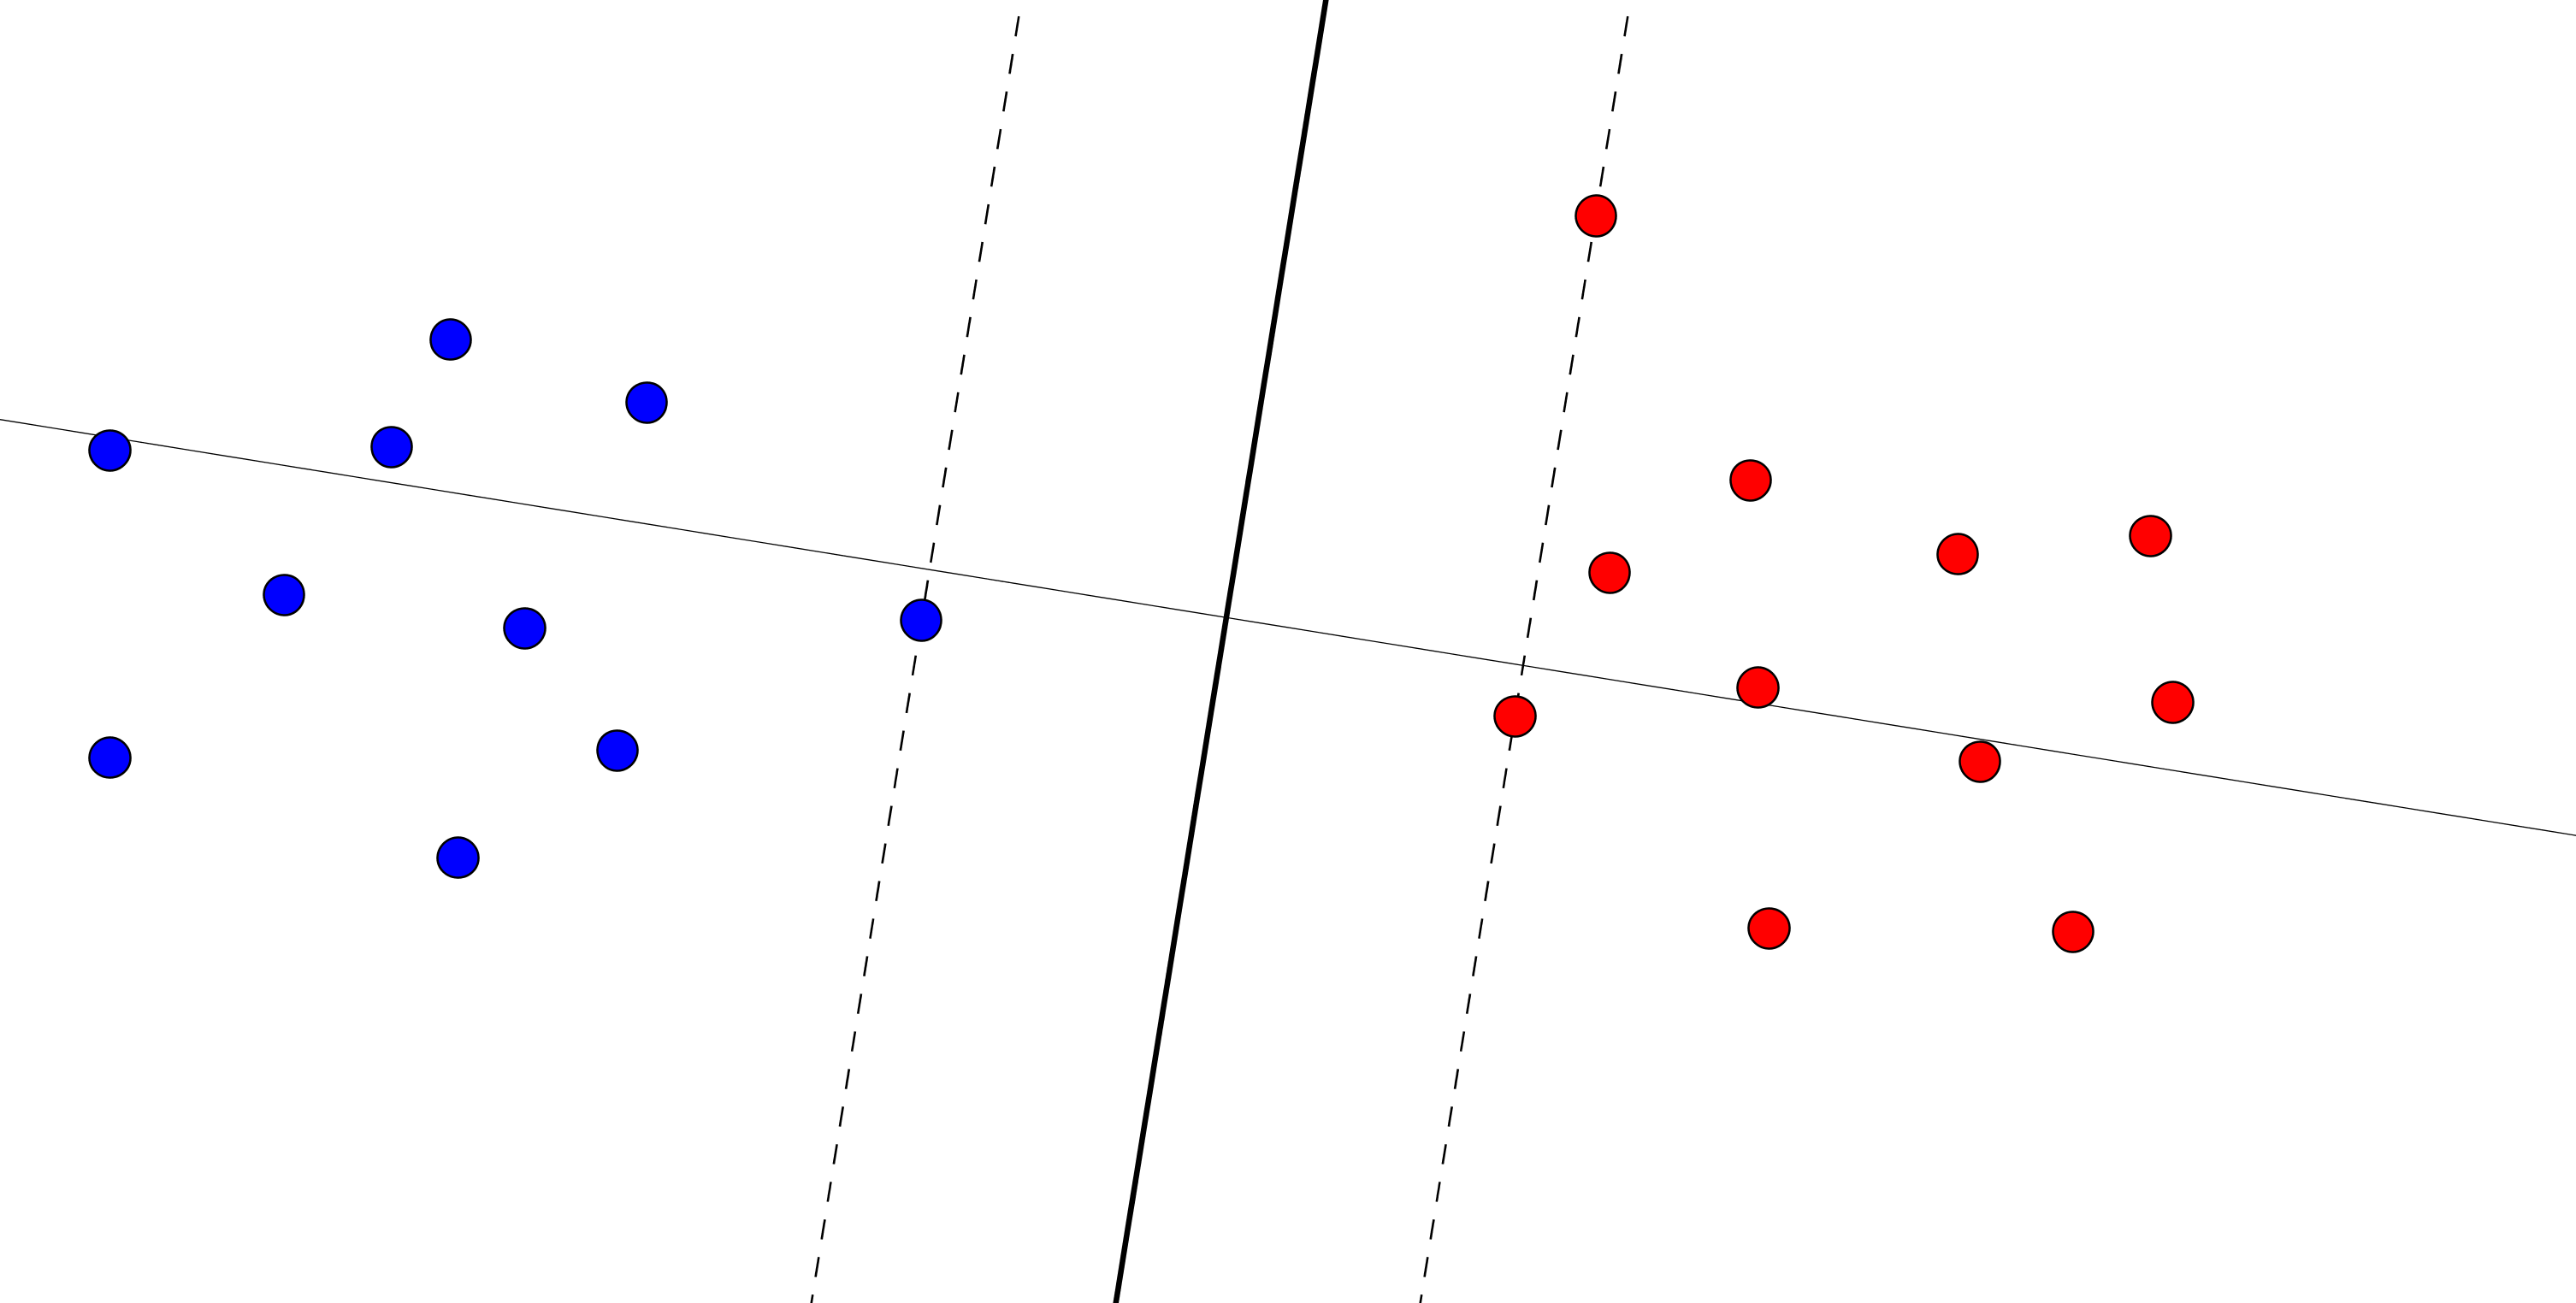
\includegraphics[width=\textwidth]{svm1.png}
\end{center}
\end{column}
\end{columns}

\vspace{5mm}
Odległość między hiperpłaszczynami wynosi: $\frac{2}{||\textbf{w}||}$, więc celem jest minimalizacja $\frac{||\textbf{w}||^2}{2}$ przy ograniczeniach:
$$
\begin{cases}
x'_i\textbf{w}+b &\geq 1\\
x'_i\textbf{w}+b &\leq -1
\end{cases}
$$
\end{frame}

\begin{frame}
\frametitle{\small PRZYPADEK DWUKLASOWY, LINIOWO NIESEPAROWALNY}
Dokładamy stałe $\xi_i\geq 0$ osłabiające warunek liniowej separowalności (kary za nieidealne rozdzielenie). W takiej sytuacji rozwiązujemy problem optymalizacyjny:
\begin{columns}
\begin{column}[t]{0.35\textwidth}
$$
\min\left\lbrace\dfrac{1}{2}||\textbf{w}||^2+C\sum_{i=1}^{n}\xi_i\right\rbrace
$$
przy ograniczeniach:
$$
\begin{cases}
x'_i\textbf{w}+b &\geq 1-\xi_i\\
x'_i\textbf{w}+b &\leq -1+\xi_i
\end{cases}
$$
\end{column}
\begin{column}[t]{0.65\textwidth}
\begin{center}
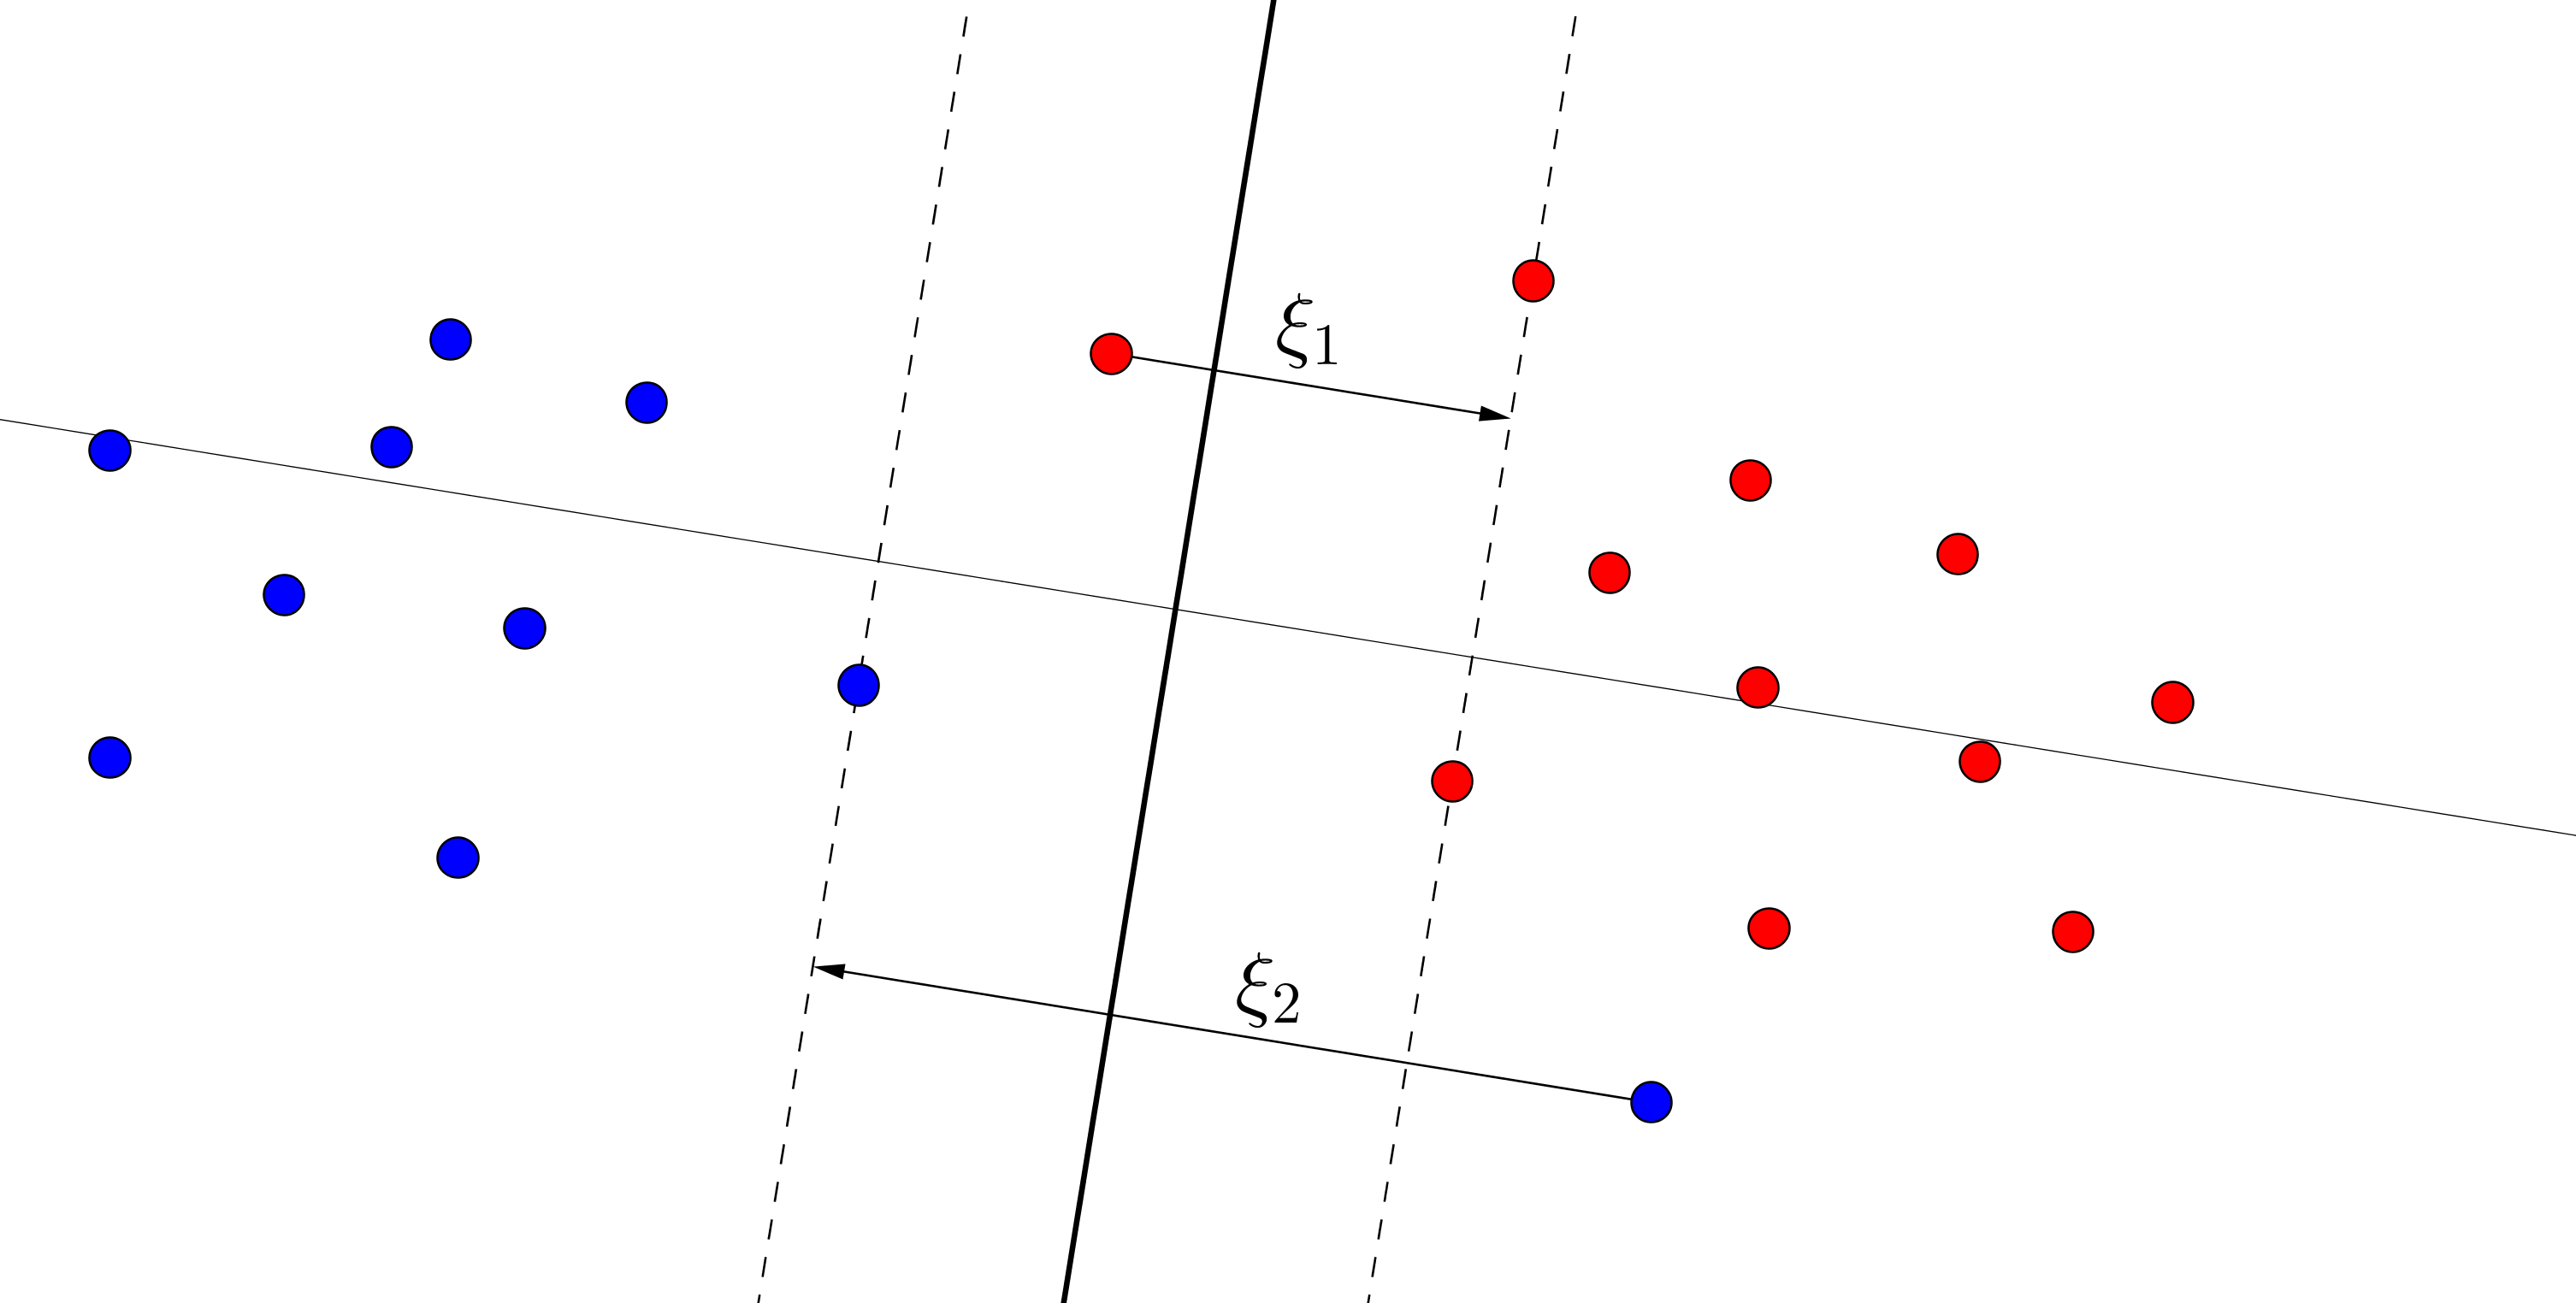
\includegraphics[width=\textwidth]{svm2.png}
\end{center}
\end{column}
\end{columns}

\end{frame}


\begin{frame}
\frametitle{\small PRZYPADEK $J$ UPORZĄDKOWANYCH KLAS}
Optymalizujemy:
$$
\min_{\textbf{w}, b_k}\left\lbrace \dfrac{1}{2}||\textbf{w}||^2+C\sum_{j=1}^{J-1}\left( \sum_{k=1}^{j}\sum_{i=1}^{n_k}\xi_{ki}^j+\sum_{k=1}^{j}\sum_{i=1}^{n_k}\xi_{ki}^{*j}\right)\right\rbrace
$$
przy ograniczeniach:
$$
\begin{cases}
\textbf{w}x_i^k-b_j&\leq -1 +\xi^j_{ki}, \hspace{6mm} \textrm{dla}\hspace{3mm} k=1,\ldots,j \hspace{3mm}\textrm{oraz}\hspace{3mm} i=1,\ldots,n_k \\
\textbf{w}x_i^k-b_j&\geq +1 -\xi^{*j}_{ki}, \hspace{6mm} \textrm{dla}\hspace{3mm} k=j+1,\ldots,J \hspace{3mm}\textrm{oraz}\hspace{3mm} i=1,\ldots,n_k 
\end{cases}
$$
\end{frame}

\begin{frame}
\centering
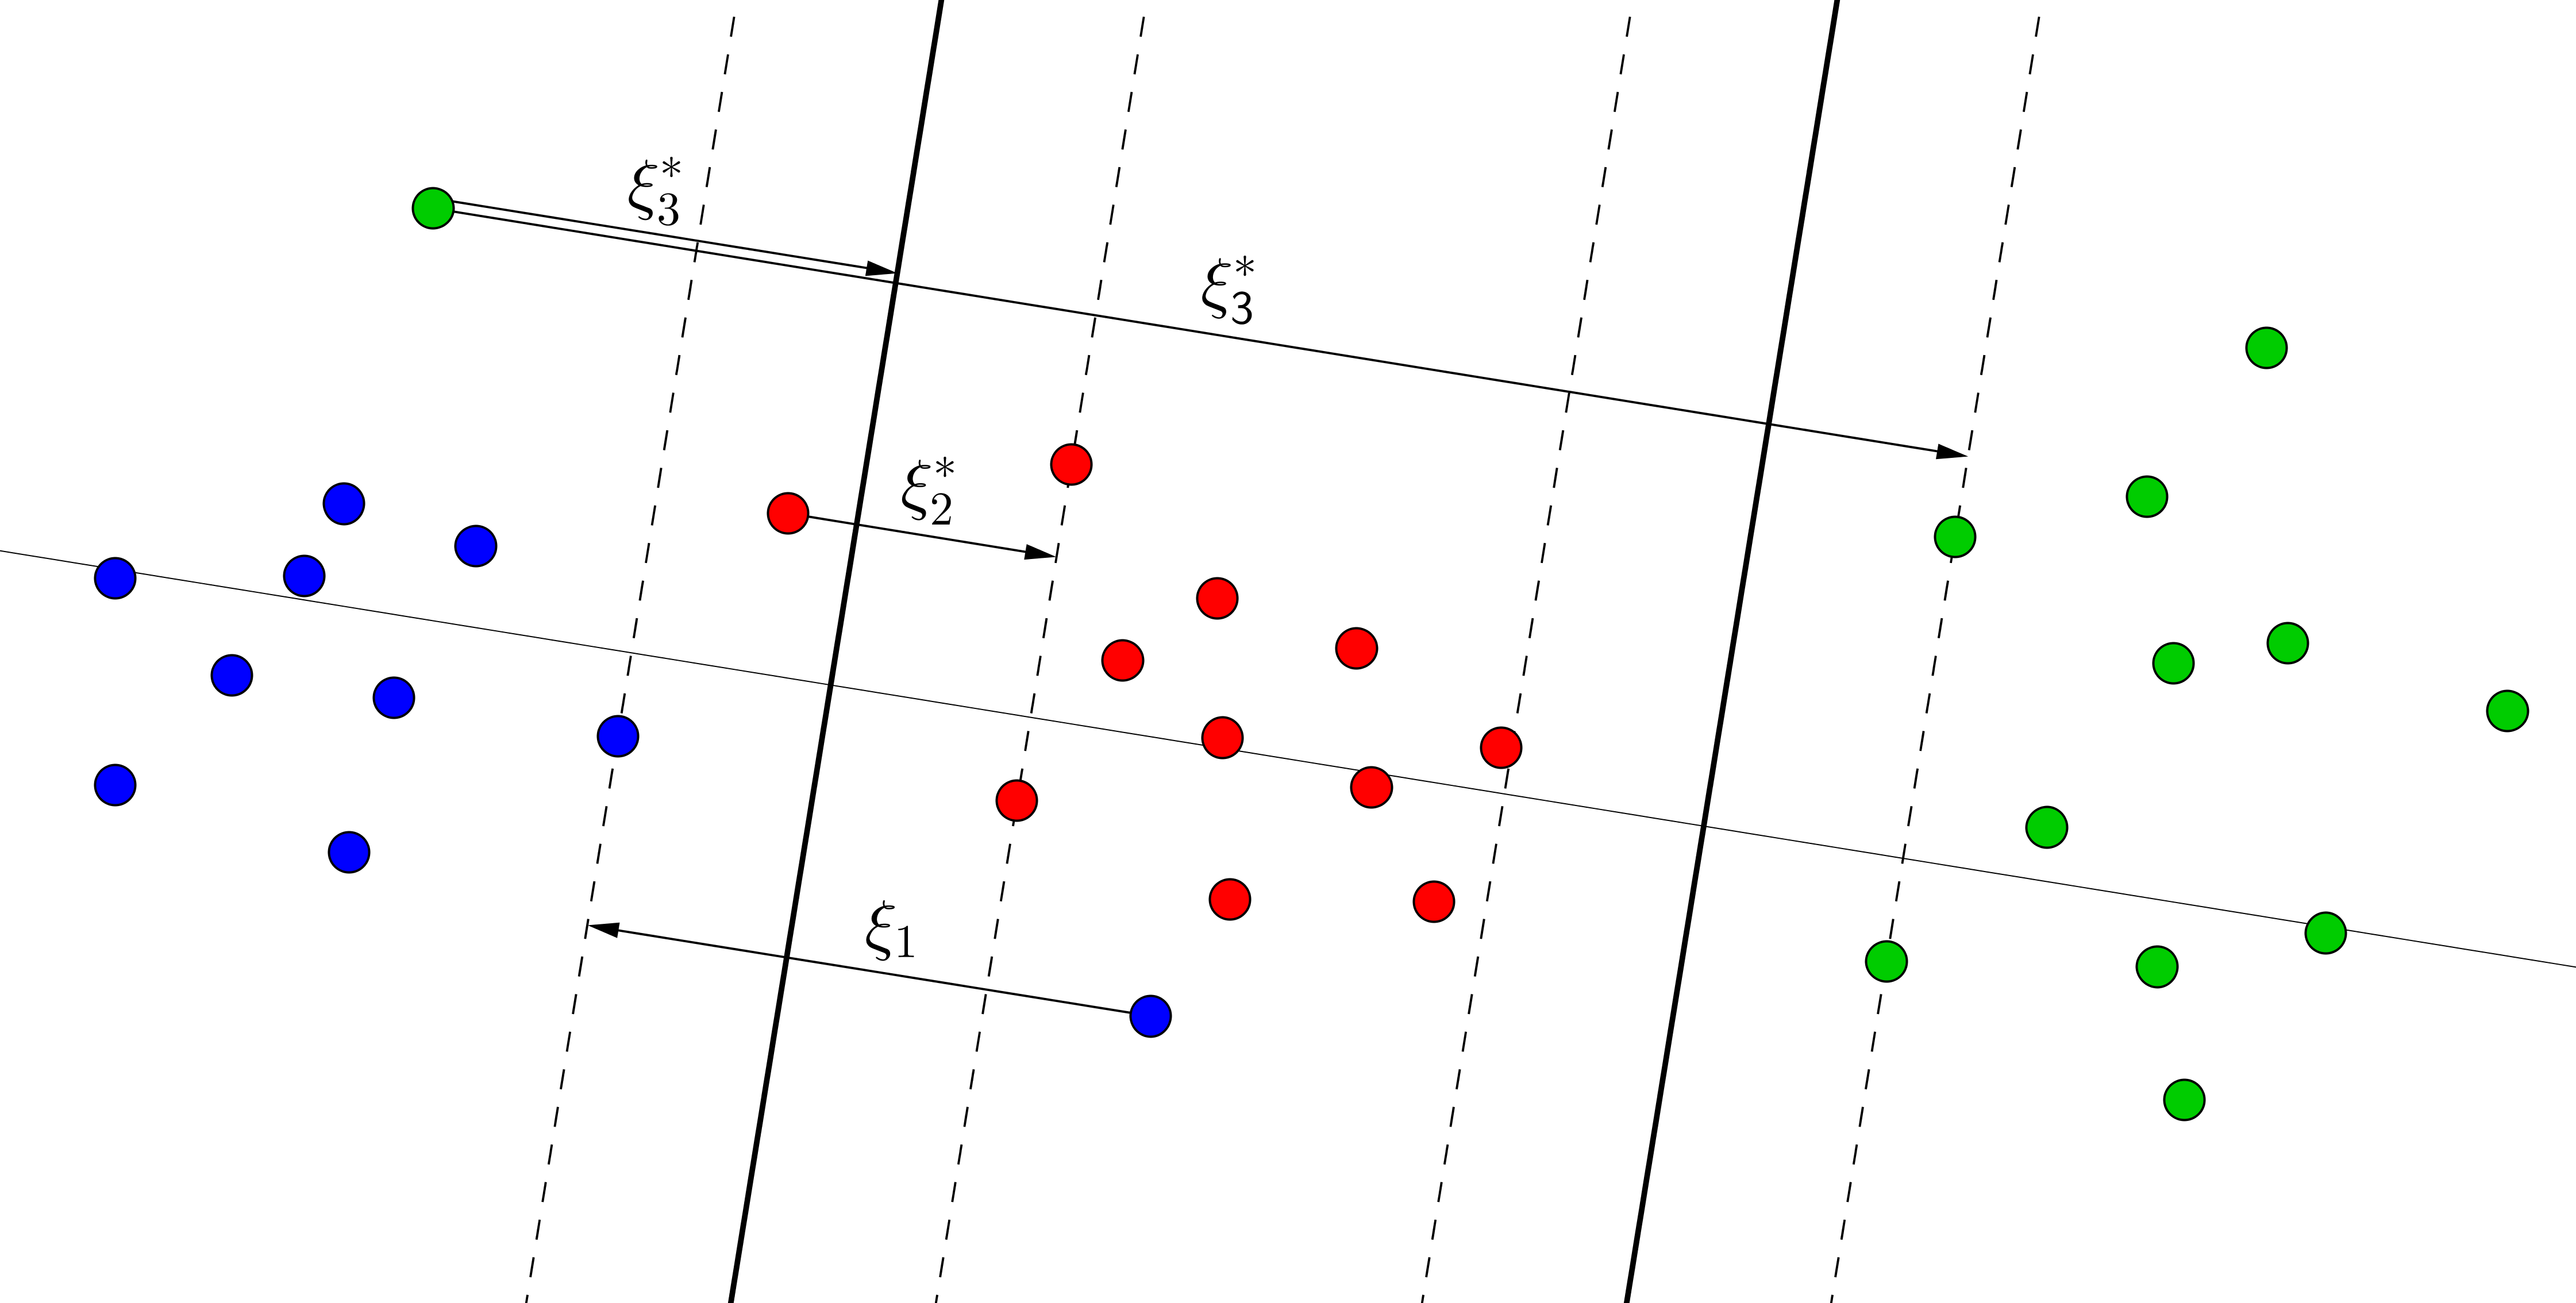
\includegraphics[width=\textwidth]{svm3.png}
\end{frame}

\begin{frame}
\Huge
\centering
\textbf{METODA ZAPROPONOWANA PRZEZ E.~FRANKA I~M.~HALLA}
\end{frame}

\begin{frame}
Podejście Franka i Halla do zagadnienia regresji porządkowej opiera się nie na stworzeniu nowego modelu, ale na odpowiednim przedefiniowaniu zbioru danych, a następnie na sprowadzeniu zadania do problemu zwykłej klasyfikacji z dwoma klasami. 

\vspace{10mm}
\begin{minipage}[c]{0.35\textwidth}
\textcolor{blue}{$J-$klasowy problem \\regresji porządkowej}
\end{minipage}
\begin{minipage}[c]{0.2\textwidth}
\centering
\Huge
\textcolor{blue}{$\longrightarrow$}
\end{minipage}
\begin{minipage}[c]{0.35\textwidth}
\flushright
\textcolor{blue}{$J-1$ dwuklasowych problemów klasyfikacji}
\end{minipage}
\end{frame}

\begin{frame}
Na czym więc polega transformacja danych? Przeanalizujmy to na~przykładzie:
\begin{eqnarray*}
\mathcal{Y}=&\lbrace&\hspace{0mm}bardzo\_sie\_nie\_zgadzam,\hspace{5mm}nie\_zgadzam\_sie,\\ && zgadzam\_sie,\hspace{5mm}bardzo\_sie\_zgadzam\hspace{3mm} \rbrace.
\end{eqnarray*}
Dzielimy $4-$klasowy problem regresji porządkowej na $3$ dwuklasowe problemy klasyfikacji w następujący sposób:
\begin{eqnarray*}
\textrm{Zbiór nr 1: }\hspace{5mm}Cel &>& bardzo\_sie\_nie\_zgadzam\\
\textrm{Zbiór nr 2: }\hspace{5mm}Cel &>& nie\_zgadzam\_sie\\
\textrm{Zbiór nr 3: }\hspace{5mm}Cel &>& zgadzam\_sie
\end{eqnarray*}
Przy czym modyfikacji ulega jedynie wektor $\mathcal{Y}$, zbiór $\mathcal{X}$ pozostaje bez zmian.
\end{frame}

\begin{frame}

\footnotesize

\uncover<1->{
\begin{center}
\begin{tabular}{c|c}
$\mathcal{X}$ & $\mathcal{Y}$ \\
\hline
$1$ $3$ $5$ A & $bardzo\_sie\_nie\_zgadzam$\\
$3$ $3$ $3$ A & $bardzo\_sie\_nie\_zgadzam$\\
$1$ $4$ $4$ F & $nie\_zgadzam\_sie$\\
$2$ $3$ $3$ A & $bardzo\_sie\_zgadzam$\\
$5$ $9$ $1$ A & $zgadzam\_sie$\\
$1$ $6$ $5$ B & $bardzo\_sie\_nie\_zgadzam$\\
\end{tabular}
\end{center}
}
\begin{center}
	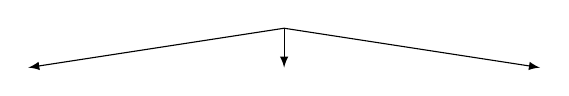
\begin{tikzpicture}[scale=0.25]
		\uncover<4->{\draw [-latex] (0, 0) -- (13, -2);}
		\uncover<3->{\draw [-latex] (0, 0) -- (0, -2);}
		\uncover<2->{\draw [-latex] (0, 0) -- (-13, -2);}
	\end{tikzpicture}
\end{center}

\begin{columns}
	\begin{column}[t]{0.3\textwidth}
		\centering
		\uncover<2->{
		\begin{tabular}{c|c} 
			\multicolumn{2}{c}{\textrm{Zbiór nr $1$:}}\\ 
			$\mathcal{X}$ & $Cel$ \\
			\hline
			$1$ $3$ $5$ A & $0$\\
			$3$ $3$ $3$ A & $0$\\
			$1$ $4$ $4$ F & $1$\\
			$2$ $3$ $3$ A & $1$\\
			$5$ $9$ $1$ A & $1$\\
			$1$ $6$ $5$ B & $0$
			\end{tabular}
		}
		
		\uncover<5->{	
		\begin{center}
			\begin{tikzpicture}[scale=0.25]
				\draw [-latex] (0, 0) -- (0, -3);
			\end{tikzpicture}
			
			\mbox{$\mathbb{P}(Cel > bardzo\_sie\_nie\_zgadzam|\underline{x})$}
		\end{center}
		}

	\end{column}

	\begin{column}[t]{0.3\textwidth}
		\centering
		\uncover<3->{
		\begin{tabular}{c|c} 
			\multicolumn{2}{c}{\textrm{Zbiór nr $2$:}}\\ 
			$\mathcal{X}$ & $Cel$ \\
			\hline
			$1$ $3$ $5$ A & $0$\\
			$3$ $3$ $3$ A & $0$\\
			$1$ $4$ $4$ F & $0$\\
			$2$ $3$ $3$ A & $1$\\
			$5$ $9$ $1$ A & $1$\\
			$1$ $6$ $5$ B & $0$
		\end{tabular}
		}
		
		\uncover<6->{
		\begin{center}
			\begin{tikzpicture}[scale=0.25]
				\draw [-latex] (0, 0) -- (0, -1);
			\end{tikzpicture}
			\mbox{$\mathbb{P}(Cel > nie\_zgadzam\_sie|\underline{x})$}
		\end{center}
		}
		
	\end{column}
	
	\begin{column}[t]{0.3\textwidth}
		\centering
		\uncover<4->{
		\begin{tabular}{c|c} 
			\multicolumn{2}{c}{\textrm{Zbiór nr $3$:}}\\ 
			$\mathcal{X}$ & $Cel$ \\
			\hline
			$1$ $3$ $5$ A & $0$\\
			$3$ $3$ $3$ A & $0$\\
			$1$ $4$ $4$ F & $0$\\
			$2$ $3$ $3$ A & $1$\\
			$5$ $9$ $1$ A & $0$\\
			$1$ $6$ $5$ B & $0$
		\end{tabular}
		}
		
		\uncover<7->{
		\begin{center}
			\begin{tikzpicture}[scale=0.25]
				\draw [-latex] (0, 0) -- (0, -3);
			\end{tikzpicture}
			
			\mbox{$\mathbb{P}(Cel > zgadzam\_sie|\underline{x})$}
		\end{center}
		}
	\end{column}
\end{columns}
\end{frame}

\begin{frame}
Następnie dostajemy nową obserwację o zmiennych objaśnianych $\underline{x}$ i chcemy dowiedzieć się, do jakiej klasy z $\mathcal{Y}$ będzie ona należała. Co robimy? Korzystając z poprzednich modeli, liczymy po kolei:

\begin{eqnarray*}
\mathbb{P}(Cel &>& bardzo\_sie\_nie\_zgadzam\hspace{2mm}|\hspace{2mm}\underline{x})\\
\mathbb{P}(Cel &>& nie\_zgadzam\_sie\hspace{2mm}|\hspace{2mm}\underline{x})\\
\mathbb{P}(Cel &>& zgadzam\_sie\hspace{2mm}|\hspace{2mm}\underline{x})
\end{eqnarray*}

\end{frame}

\begin{frame}
Kolejne prawdopodobieństwa wylicza się łańcuchowo. Mianowicie:

\begin{footnotesize}
\begin{align*}
\uncover<2->{
\mathbb{P}(Cel = bardzo\_sie\_nie\_zgadzam\hspace{0.5mm}|\hspace{0.5mm}\underline{x})& =&&1-\mathbb{P}(Cel > bardzo\_sie\_nie\_zgadzam\hspace{0.5mm}|\hspace{0.5mm}\underline{x})\\
}\uncover<3->{
\mathbb{P}(Cel = nie\_zgadzam\_sie\hspace{0.5mm}|\hspace{0.5mm}\underline{x})&=&&\mathbb{P}(Cel > bardzo\_sie\_nie\_zgadzam\hspace{0.5mm}|\hspace{0.5mm}\underline{x}) - \\
& &&\mathbb{P}(Cel > nie\_zgadzam\_sie\hspace{0.5mm}|\hspace{0.5mm}\underline{x})\\
}\uncover<4->{
\mathbb{P}(Cel = zgadzam\_sie\hspace{0.5mm}|\hspace{0.5mm}\underline{x})&=&&\mathbb{P}(Cel > nie\_zgadzam\_sie\hspace{0.5mm}|\hspace{0.5mm}\underline{x}) - \\
& && \mathbb{P}(Cel > zgadzam\_sie\hspace{0.5mm}|\hspace{0.5mm}\underline{x})\\
}\uncover<5->{
\mathbb{P}(Cel = bardzo\_sie\_zgadzam\hspace{0.5mm}|\hspace{0.5mm}\underline{x})& =&&\mathbb{P}(Cel > bardzo\_sie\_zgadzam\hspace{0.5mm}|\hspace{0.5mm}\underline{x})}
\end{align*}
\end{footnotesize}

\uncover<6->{Ostatecznie, naszej nowej obserwacji przypisujemy klasę z~maksymalnym prawdopodobieństwem.}
\end{frame}

\begin{frame}
\Huge
\centering
\textbf{KRZYWA ROC I WSPÓŁCZYNNIK AUC}
\end{frame}

\begin{frame}
\frametitle{PRZYPADEK DWUKLASOWY}
\vspace{2mm}
\begin{columns}
\centering
	\begin{column}[c]{0.5\textwidth}
		\begin{tabular}{cc|cc} 
			& & \multicolumn{2}{c}{$Klasa$}\\ 
			& & $1$ & $0$ \\
			\hline
			\multirow{2}{*}{$\widehat{Klasa} $}
			& $1$ & TP & FP\\
			& $0$ & FN & TN
		\end{tabular}
	\end{column}
	\begin{column}[c]{0.5\textwidth}		
		\begin{eqnarray*}
		TPR&=&\dfrac{TP}{TP+FN}\\
		FPR&=&\dfrac{TN}{FP+TN}		
		\end{eqnarray*}
	\end{column}
\end{columns}	
\centering

\begin{table}[h]
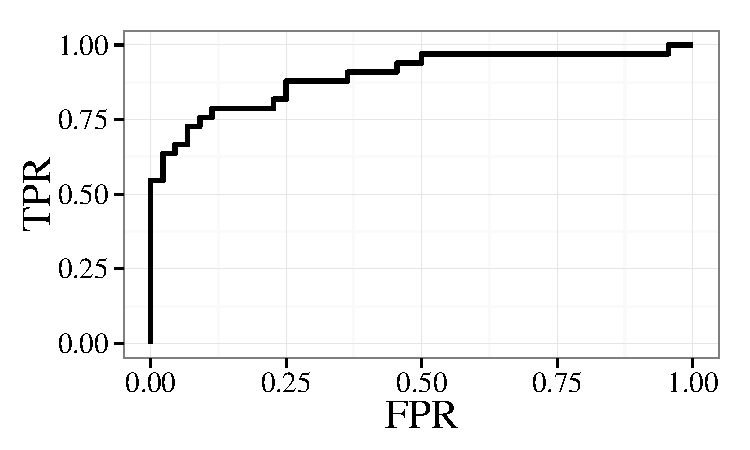
\includegraphics[scale=0.6]{roc3.pdf}
\caption{Przykładowa krzywa ROC}
\end{table}

\end{frame}

\begin{frame}
\frametitle{PRZYPADEK KLASYFIKACJI PORZĄDKOWEJ}
\centering
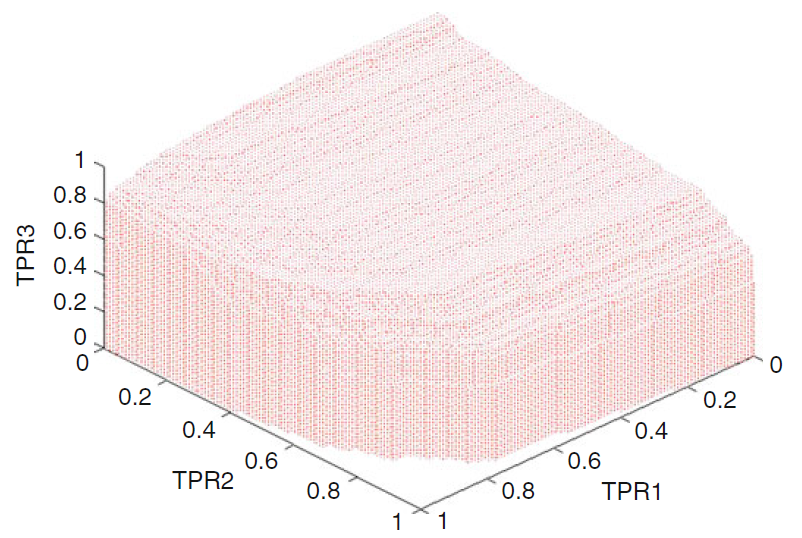
\includegraphics[scale=0.4]{roc3d.png}

$$
VUS = \dfrac{1}{\prod_{k=1}^J n_k}\sum_{y_{j_1}<\ldots<y_{j_J}} \mathbb{I}_{f(x_{j_1})<\ldots<f(x_{j_J})}
$$

\end{frame}



\begin{frame}
	\frametitle{Bibliografia}
	\begin{thebibliography}{9}
		\bibitem{} Frank E., Hall M., A simple approach to ordinal classification, \emph{Proceedings of the European Conference on Machine Learning}, Freibourg, Niemcy, 2001, str. 146--156.
		\bibitem{} Waegman W., De Baets B., A survey on ROC-based ordinal regression, w: Fürnkranz J., Hüllermeier E. (Eds.), \emph{Preference Learning}, Springer, 2010, str. 127-154.
	\end{thebibliography}
\end{frame}

\end{document}
